
\documentclass{article}% use option titlepage to get the title on a page of its own.

\linespread{1.4}

\usepackage{lmodern}
\usepackage{listings}
\usepackage{color}

\definecolor{dkgreen}{rgb}{0,0.6,0}
\definecolor{gray}{rgb}{0.5,0.5,0.5}
\definecolor{mauve}{rgb}{0.58,0,0.82}

\usepackage{graphicx}
\graphicspath{ {./images/} }



\title{%
  Non-negative LASSO \\
  \large A Portfolio replication application}

\date{2019, February}
\author{Giovanni Misseri, Andrea Della Vecchia \\ \\ 
Business Economics and Finantial Data}
\begin{document}
\maketitle
\tableofcontents
\newpage
\section{Introduction}

Portfolio management has always been one of the most used way investors start approaching to financial investments. An important task in finance is indeed optimizing the revenue with respect to the risk of investing in a portfolio.

Markowitz in the '50, stated that single minded pursuit of high returns results in a poor strategy and rational investors need to balance their desire for high returns with low risk. So investing in a portolio seems reasonable, indeed it diversify our investment and if we are able to spot profitable companies on which invest, we are guaranteed good revenue taking relatively low risk.
\\

There are mainly two stratgies in portfolio management, active and passive managements. Active management tries to exploit the fluctuations of the market to gain as much as possible. On the other hand, passive management, tries to mimic the performance of an index. As one can easily notice, with active approach it's possible to loose great amount of money even investing on, on average, growing companies. On the other hand if we are able to well mimic a, on average, growing index, with passive approach we are guaranteed positive revenue.

Empirically is often the case passive approach outperforms active approach, also due to the transaction costs. In this work will try to propose two different solution to pursue respectively the passive and the active approach.

\newpage
\section{Shrinkage Methods}

If we have a feature or some mesurements of an interesting phenomenon, is often the case that, given some related variables, we try to explain the phenomenon as a function of the related variables. The use of linear model, in case of linear relation between phenomenon and variables, is a good choise for two reasons: it gives good prediction and on the other hand, given the linear relation, it's highly intrpretable. 

In general the more correlated variables we have, the "better" the model will be; but sometimes the presence of too much independent variables conditions the prediction error and also the presence of an high number of predictors limits the interpretability of the model. For these reasons one could decide to add a regularization term to its minimum least square problem.

\[
\min_{\beta_0 , \beta} \frac{1}{N} \sum_{i=1}^N (y_i-\beta_0 - \sum_{j=1}^p x_{ij}\beta_j)^2 + \lambda\sum_{j=1}^p |\beta_j |^q 
\]

Where $|\beta|^p$ is the $p$-norm of $\beta$.
\\

If in the regularized minimization problem we choose norm-two we obtain the ridge regression, if we choose the norm-one we obtain LASSO regression. 


It's easy to proove that shrinkage methods also solve an other tipe of problem related to ordinary least square. With OLS indeed the solution of the minimization problem is $ \beta_{ols}=(X^TX)^{-1}X^Ty$, decomposing $X$ through SVD, $X=V\Sigma U^T$, we get $\beta_{ols}=U\Sigma^{-1}V^Ty$. From this we can easly see that if $\Sigma$ is not invertible $\beta_{ols}$ could not be found.
\\

Shrinkage methods deal with this problem. Ridge regression ends up giving $\beta_{ridge}=U(\Sigma^2+\lambda I)^{-1} \Sigma V^T y$. Lasso regression's beta cannot be written in an explicit form, but the non-invertibility problem is solved due to the fact that, fixed $\lambda$, at the optimum, some beta will be equal to zero. Intuitivelly this is due to the feasible solutions space shape; indeed LASSO regression can be written as the following minimization problem.
\begin{equation}
 \min_{\beta} \sum_{i=1}^N ( y_i -\beta_0 -\sum_{j=1}^p x_{ij} \beta_j)^2 ~~subject~to~\sum_{j=1}^p |\beta_j| \leq t
\end{equation}

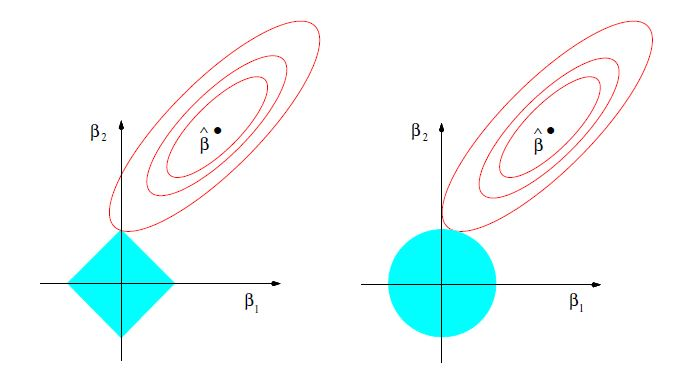
\includegraphics[scale=0.75]{lasso}

\subsection{LASSO and Portfolio Replication}

A replicating portfolio for a given asset or series of cash flows is a portfolio of assets with the same properties. So the principal problem of building a good replicating portfolio for a certain financial aggregate index is finding the right componets of the index, the one able to represent the index itself. 

With the problem posed like that, the link between lasso regression and portfolio replication it's evident. Indeed one interesting properties of lasso regression is the variable selection consistency, so using lasso regression we are guaranteed, under certain condition, that it will select an optimal subset of variables in order to explain our dependent variable. It's clear now that lasso could help on the selection of the subset of time series that will be part of the portfolio; so we will select a subset of an index' components  able to explain the index itself.
\\

Here comes one problem, how to use lasso, a cross-sectional regression method, on a dynamic dataset? We will use a moving window approach, so we will assume that the data inside a window of fixed lenght are time invariant, and we compute lasso on that.

Another problem is the interpretation of the resulting model. Ones we find the solution to the lasso minimization problem, we have the beta related to all the variables, in our case the components of the index. Some beta will be equal to zero, so they will be excluded by our portfolio, for all the other beta a nice interpretation is available. 

If we carefully think to lasso as it has been defined in $(1)$, we approximate an index, the used one will be $Sp500$, as a function of some of it's components, conditioning to the fact that the sum of the associated beta is less than a given $t$. Practically we will work on the daily log-retuns, and so our response and regressor will be all daily log-return; said that it's easy to see that $t$ can be seen as the initial budget and each beta is the volume of the "suggested" investment in a certain asset. Later on we will exploit this fact to run simulations using the different proposed methods.

For an active approach everithing works fine, a positive beta will be an investment and a negative beta will be a short sell. On the other hand, for passive approach, it could be forbidden or in general doesn't make much sense to use short sell. For this reason to our estimates we need to add the constrain of non-negativity.
\\

Considering that also elastic net regression has the consistency variable selection, we will try to select the assets both with lasso and elastic net regression. Some comparison will be done on that.

\subsection{Parameter estimation}
As we said our principal aim is to replicate the $Sp500$ with a relatively low number of assets. To select the rigth one we could use, as explained in the previous paragraph, lasso or elastic net regression; now we have to deal with the parameter estimation.

As we said we suppose, as actually happend due to the fact that our index is just a combination of 500 assets, that $Sp500$ has a linear relation with the selected assets. A first and natural choise for the $\beta$ of the model are the one obtained by the non-negative lasso regression or non-negative elastic net regrssion on the whole set of $Sp500$ constituents. Actually this gives nice results, but we will see in experimental phase that selecting the assets and than estimate the model using OLS works better. 















\newpage
\section{Portfolio replication}





\end{document}